\documentclass[12pt]{article}
\usepackage{amsmath}
\usepackage{graphicx}
\usepackage{fullpage}
\usepackage{algorithm}
\usepackage{algorithmicx}
\usepackage[noend]{algpseudocode}
\usepackage{xcolor}

\title{Assignment 3 Solutions}
\author{COMP 3804, Fall 2018 \\
	Michael Kuang 101000485}
\date{November 19, 2018}
\begin{document}
\maketitle

\newpage

\section{Problems}

\begin{enumerate}
\item Find strongly connected components of the graph in the Figure.

\begin{center}

\end{center}

% Question 2

\item \color{blue} Let $G=(V,E)$ be a directed graph. We say that $G$ is {\em semi-connected} if for every pair of distinct vertices $u,v\in V$,  we have that there is a directed path from $u$ to $v$ or there is a directed path from $v$ to $u$ in $G$.  Given $G$ in the adjacency list representation, design an algorithm running in $O(|V|+|E|)$ time to determine whether $G$ is semi-connected. Note that this is similar to the question which we had in the mid-term, where we needed to check whether a directed acyclic graph is semi-connected.  As a hint, again design an algorithm for the directed acyclic graphs. Think of a general directed graph, in terms of directed acyclic graphs of its strongly connected components. [Consult Section 3.4 of the text-book.] 
Is the graph in the above Figure semi-connected?


\color{black}
\textbf{Solution}\\
The SCC() function returns the strongly connected components of the graph.
The DFS() function does a depth-first search in the graph, labelling the post numbers for each vertex.
The TopologicalSort() function topologically sorts and returns the vertices starting from the largest post number in decreasing order.

\begin{algorithm}
\caption{Determining if $G$ is semi-connected}
\begin{algorithmic}[1]
\Procedure{IS-SEMICONNECTED}{$G$}
	\State $G'\gets SCC(G)$ \Comment{Obtain a SCC from graph G}
	\State $DFS(G')$ \Comment{DFS G', labelling the post numbers}
	\State $VSorted \gets TopologicalSort(G')$ \Comment{Return topologically sorted array of vertices}
	\For{i = 0 to length(VSorted) - 2}
		\If{$(VSorted[i], VSorted[i+1]) \not\in\ G.E$}
			\State Return False
		\EndIf
	\EndFor
	\State Return True
\EndProcedure
\end{algorithmic}
\end{algorithm}

\textbf{Proof of Correctness}\\
Suppose that the SCC(), DFS() and TopologicalSort() are correct. In order to determine if the graph is {\em semi-connected}, we observe that for each vertex in the topologically sorted array, it must have a directed edge to the next vertex in that sorted array. So, assume that we have a topologically sorted array $VT= (v_1, v_2, v_3, ... v_n)$ of graph $G$, then the edge$(v_i, v\textsubscript{i+1}) \in G.E$ for the graph to be {\em semi-connected}, otherwise it is not.
\\
\textbf{Time Complexity Analysis}\\

%Question 3
\item \color{blue} This question is based on the {\em cut lemma} for minimum spanning trees. Let $G=(V,E)$ be a connected graph where each edge has a positive weight. If for any cut of $G$, there is a unique edge in the cut of minimum weight then show that minimum spanning tree of $G$ is unique. Show that the converse may not be true using an example. I.e.,  construct a graph $G$ that has a unique minimum spanning tree, but there are cut(s) in $G$ containing multiple edges  having the minimum weight. However, if the cut in $G$ contains multiple edges having minimum weights, then this is not true as shown in the following figures. 

\color{black}
\textbf{Solution}\\
Let's assume for a contradiction that the graph $G$ has a unique minimum spanning trees $T$. Let $(u,v)$ be an edge in $T$. Removing edge $(u,v)$ cuts the tree $T$ into two components. Consider the cut $(u, v)$ and let $(x,y)$ be the unique minimum edge crossing the cut. If $(x,y) \neq (u,v)$ then $w(x,y) < w(u,v)$ and the spanning tree $T - \{(u,v)\} \bigcup \{(x,y)\}$ has a better cost than $T$ which leads to a contradiction because if $T$ was originally an MST, then by definition the edge $(u,v)$ should be the minimum edge that is part of $T$.  \\
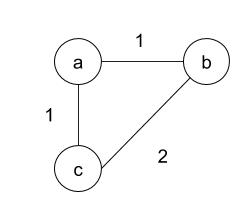
\includegraphics[scale=0.5]{q3}\\
Conversely, if we consider the graph above, there is a unique MST that contains edges $(a,b)$ and $(a,c)$, however the cut $(\{a\}, \{b,c\})$ doesn't have a unique minimum edge crossing the cut.
%Question 4
\newpage
\item \color{blue} Consider a connected graph $G=(V,E)$ where each edge has a non-zero positive weight. Furthermore, assume that all edge weights are distinct.
Using the cut property, first show that that for each vertex $v\in V$, the edge incident to $v$ with
minimum weight belongs to a Minimum Spanning Tree (MST). 
Can you use this to devise an algorithm for MST - the above step identifies at least $|V|/2$ edges in MST - you can collapse these edges, by identifying the vertices and then recursively apply the same technique - the graph in the next step has at most half of the vertices that you started with - and so on. 
What is the running time of your algorithm?\\
Note that for an edge $e=uv$ in the graph $G=(V,E)$, {\em identifying} vertex $u$ with $v$ or {\em collapsing} $e$  is the following operation: Replace the vertices $u$ and $v$  by a new vertex, say $u'$. Remove  the edge between $u$ and $v$.  If there was
an edge from $u$ (respectively, $v$) to any vertex $w$ ($w\not=u$ and $w\not=v$), then we add an edge (with the same weight as of edge  $uw$ (respectively,  $vw$)), between the vertices $u'$ and $w$. This transforms graph $G$ to a new graph $G'=(V',E')$, where $|V'|<|V|$ and $|E'| < |E|$. Note that $G'$ may be a multigraph (i.e., between a pair of vertices, there may be more than one edge). For example, if $uv$,  $uw$,  and  $vw$ are edges in $G$, then $G'$ will have two edges between $u'$ and $w$ when we identify $u$ with $v$. We can transform $G'$ to a simple graph by  keeping  the edge with the lower weight among $uw$ and $vw$ as the representative for $u'w$ for the computation of MST.

\color{black}
\textbf{Solution} 
\begin{algorithm}
\caption{Finding MST}
\begin{algorithmic}[1]
\Procedure{MST}{$G$}
	\State $F \gets G.V$ \Comment{Initialize F as a set of one-vertex trees, one for each vertex of the graph}

	\While{$F$ has more than 1 component}
		\State Determine the connected components of $F$ and label each vertex of $G$ by its component
		\State Initialize the minEdge for each component of $F$ to be $\infty$
		\For{each edge($u$, $v$) in $G$}
			\If{$ComponentLabel(u) \neq ComponentLabel(v)$ }
				
				\If{$edge(u,v) <$ the minEdge of component of  $u$ }
					\State Set $edge(u,v)$ as minEdge for the component of $u$
				\EndIf
				\If{$edge(u,v) <$ the minEdge of component of  $v$ }
					\State Set $edge(u,v)$ as minEdge for the component of $v$
				\EndIf
			\EndIf
		\EndFor
		\For{each component in $F$}
				\State Add minEdge(component) to $F$
		\EndFor			
	\EndWhile

	\State Return $F$
\EndProcedure
\end{algorithmic}
\end{algorithm}

The cut property states that given any cut in an edge-weighted graph with distinct weights, the crossing edge of minimum weight is in the MST of the graph. A crossing edge is an edge that connects a vertex in one set of the cut with a vertex in the other set of the cut and so if we add more than 1 crossing edge, this will create a cycle. 

\item \color{blue} Suppose you are given a set $S$ of $n$ distinct points in the plane.   Let $A$ and $B$ represents a partition of $S$, i.e. $A\subset S$, $B\subset S$, $S=A\cup B$, and $A\cap B=\emptyset$. Define the distance between $A$ and $B$, denoted by  $d(A,B)$, as the minimum among Euclidean distances between pair of points, where one point is from  $A$ and the other from $B$, i.e. 
$$d(A,B)=\min_{a\in A, b\in B}|ab|$$  
Our task here is to find a partition of $S$ into two non-empty sets $A$ and $B$ that maximizes $d(A,B)$. For this, we define a complete graph $G=(V,E)$ on $n$ vertices and ${n\choose 2}$ edges on these points as follows. Each vertex in $V$ represents a distinct point of $S$, and there is an edge between every pair of (distinct) vertices, where the weight of an edge 
$e=(u,v)$ is Euclidean distance between the points corresponding to $u$ and $v$. Consider a minimum spanning tree $T$ of $G$. Let $e$ be the most expensive edge in $T$ (i.e. $e$ is the last edge added to $T$ by Kruskal's algorithm). Let $V_1$ and $V_2$ be the two sets of vertices in the connected components obtained after the removal of $e$ from $T$. Show that the points  corresponding to $V_1$ and $V_2$ forms the required partitioning of $S$.       (Recall that Euclidean distance between  two points  $a=(3,5)$ and $b=(4,2)$ is $|ab|=\sqrt{(3-4)^2+(5-2)^2}= \sqrt{10}$.) 

\color{black}
\textbf{Solution} 

\item Let $G=(V,E)$ be a connected simple graph, where each edge has a weight of $3$. Devise an algorithm, running in $O(|V|+|E|)$ time, for computing shortest path distances from a specific vertex $s\in V$ to all other vertices of $G$. 
\newpage

\item Prove that the distance values extracted from the heap (priority queue) over the entire execution of Dijkstra's single source shortest path algorithm, in a directed connected graph with positive edge weights, is a NON-Decreasing 
sequence.  Where is this fact used in the correctness of the algorithm?

\item In the summer vacation, you decided to travel to various communities in Northern Canada by your favorite ATV (All-Terrain Vehicle).
%Assume that your chosen ATV can travel on all types of terrain (including lakes/swamp/ice/fly!). 
Each of the communities you want to visit is
represented as a vertex in your travel graph (a total of $|V|$ communities). Moreover, you are provided with distances between  all pairs of  communities. Think of your input graph as a complete graph (i.e. every pair of vertices are joined by an edge), and the weight of an edge, say $e=(uv)$ is the distance
between the community $u$ and $v$. Since this is in far North, and the routes between communities are not used that often, the gas stations 
are only located in communities (there are absolutely no gas stations which are outside a community). Furthermore, we can assume
that each community has at least one gas station. Once you completely fill up the tank of your ATV, it has an upper limit, say of $\Delta$ kilometers, which it can travel, and to travel any further it needs to fill up (which means at that point it needs to be in a community!).
You need to answer the following two questions

\begin{enumerate}
\item First design a method, running in $O(|V|+|E|)$ time, which can answer whether is there some path which your ATV can take, so that 
you can travel between two particular communities, say $s$ and $t$. It is obvious that if the distance between $s$ and $t$ is at most $\Delta$, then you can travel directly without refuelling. Otherwise, you can travel between $s$ and $t$, provided there are communities where we can
refuel and proceed. [For fun you may like to see whether you can travel from La Loche (in Sask.) to Mandorah (in Northen Territories), when your ATV with full tank can travel at most 100 Kms.]

\item Design an algorithm running in $O(|E|\log |V|)$ time to determine the smallest value of $\Delta$, which will enable you to travel from $s$ to $t$. (Please present Pseudocode, correctness, analysis) and use the algorithms discussed in the class/book as black boxes).
\end{enumerate}

\end{enumerate}

\end{document}